%!TEX root = ../template.tex
%%%%%%%%%%%%%%%%%%%%%%%%%%%%%%%%%%%%%%%%%%%%%%%%%%%%%%%%%%%%%%%%%%%%
%% annex.tex
%% NOVA thesis document file
%%
%% Chapter with example of appendix with a short dummy text
%%%%%%%%%%%%%%%%%%%%%%%%%%%%%%%%%%%%%%%%%%%%%%%%%%%%%%%%%%%%%%%%%%%%

\typeout{NT FILE annex.tex}

\chapter{Annex 1 - Extra figures} \label{annex_1}
\label{ann:lorem_ipsum1}

This annex is used to present the extra figures that were mentioned during the discussion of results in Section \ref{results:inf_diss}. These figures contain a summarized view of the obtained results regarding the conducted information dissemination experiments.

\begin{landscape}

\begin{figure}[htbp]
    \centering
    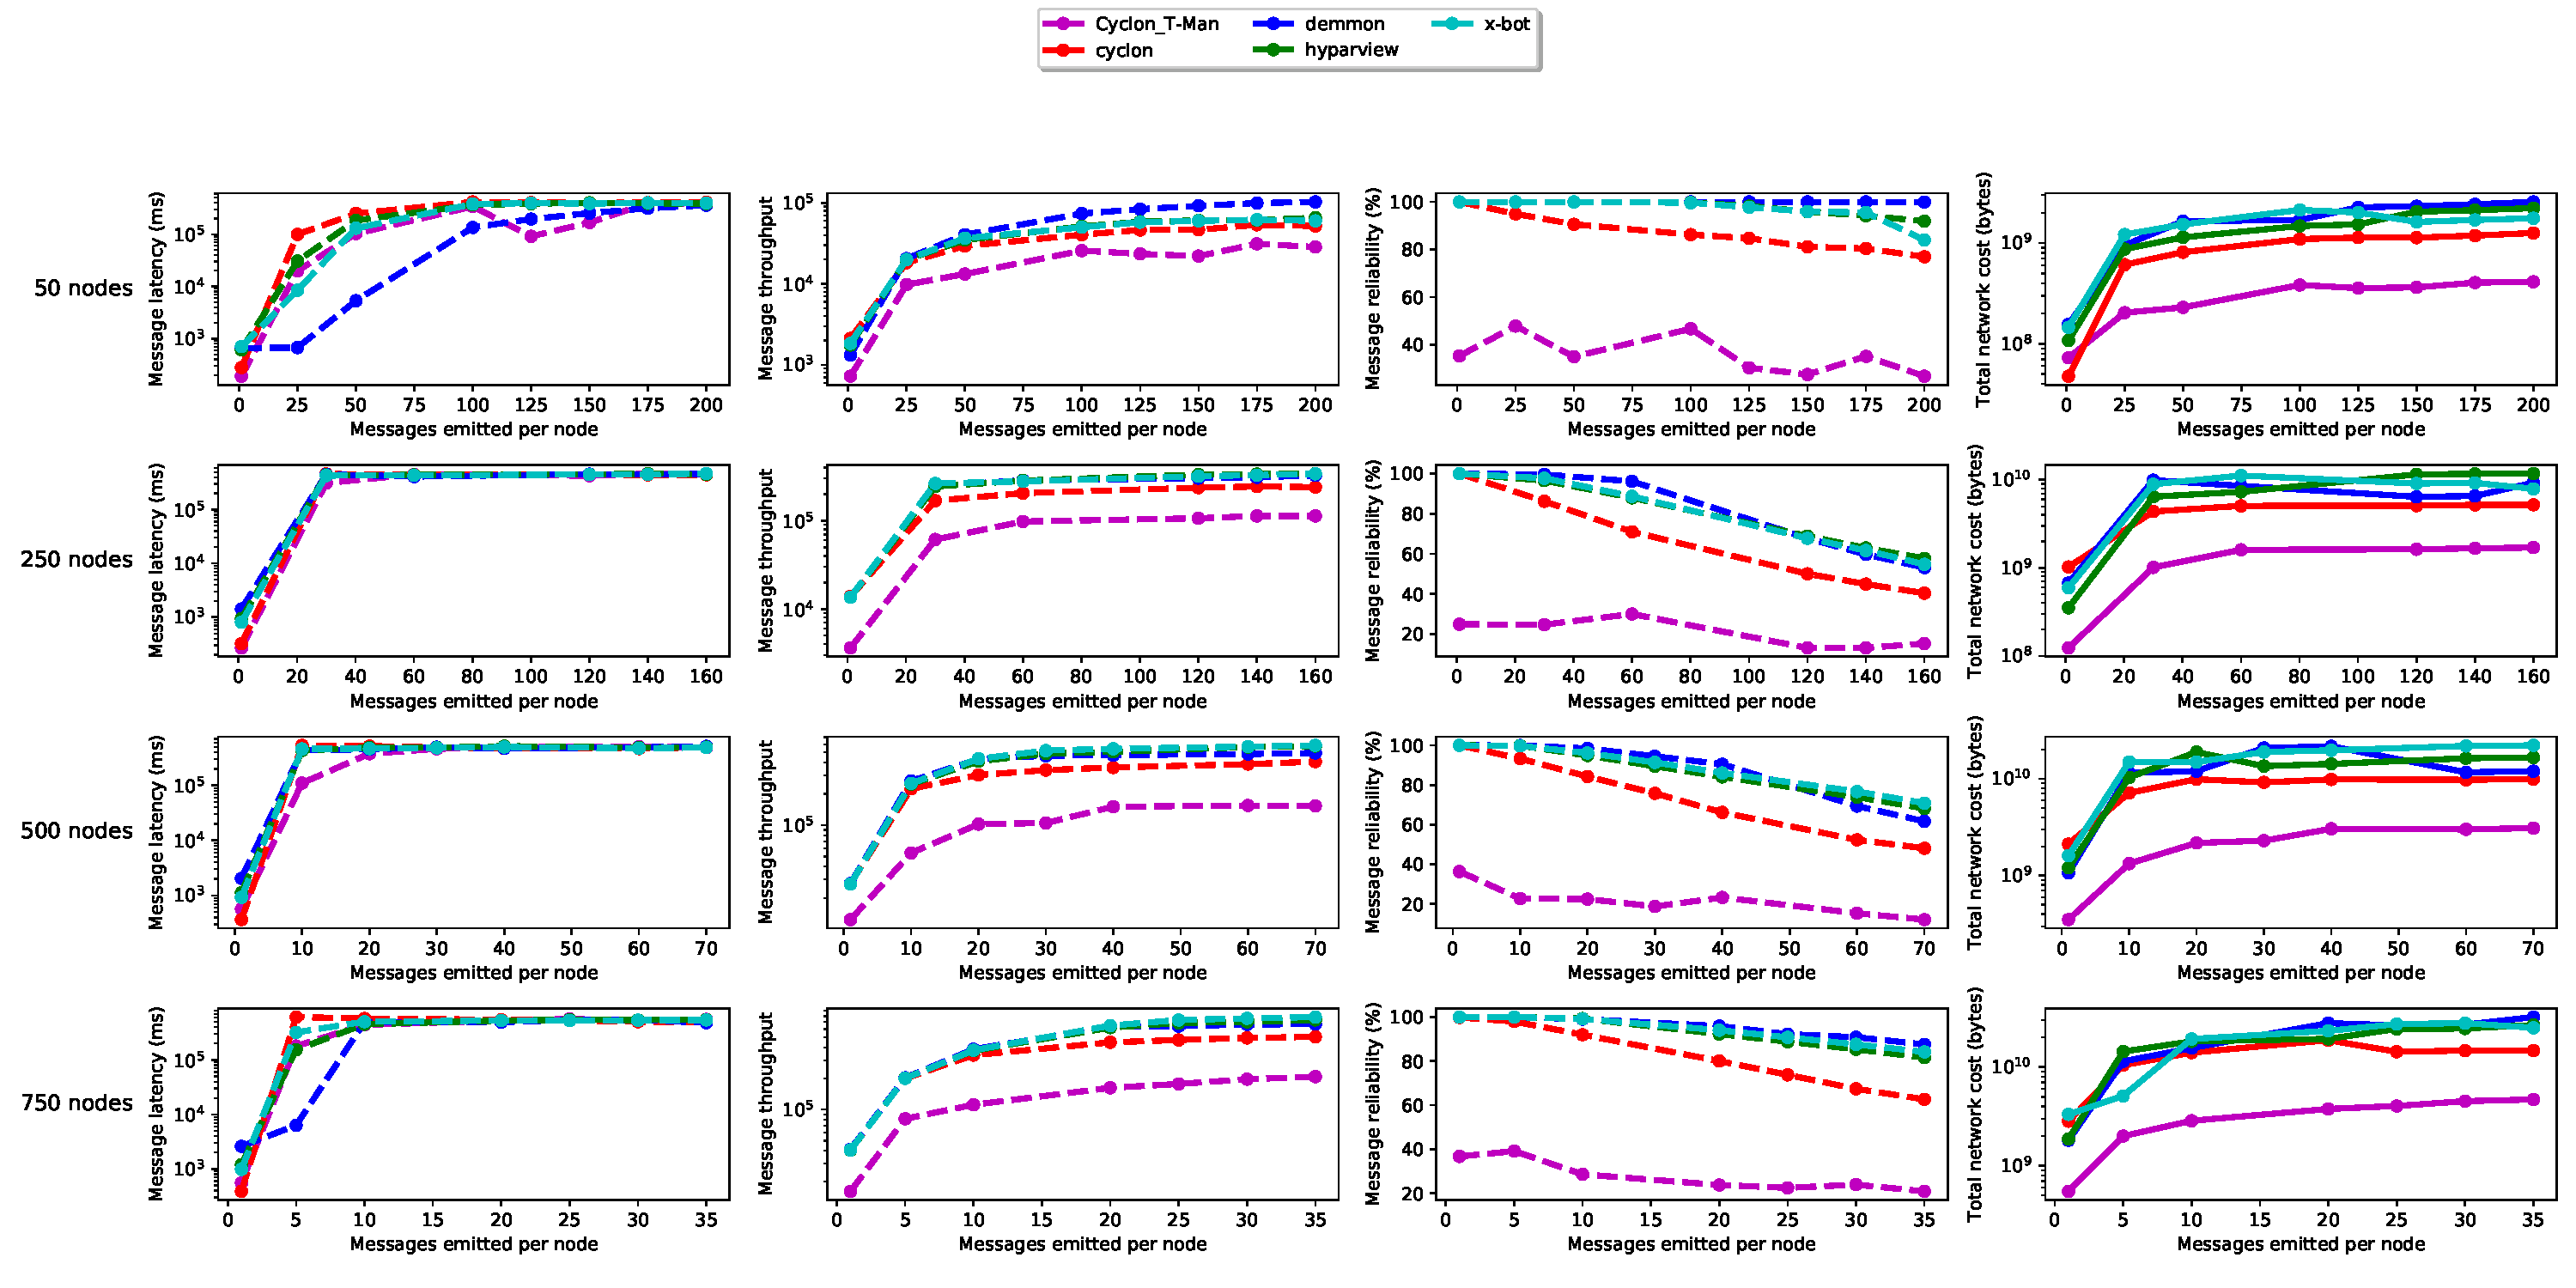
\includegraphics[width=\columnwidth]{Chapters/evaluation/figures/flood/flood_0.0_failures.pdf}
    \caption{Obtained results in simple flood scenario (0\% failures)}
    \label{fig:pouchbeasts-overview}
\end{figure}

\begin{figure}[htbp]
    \centering
    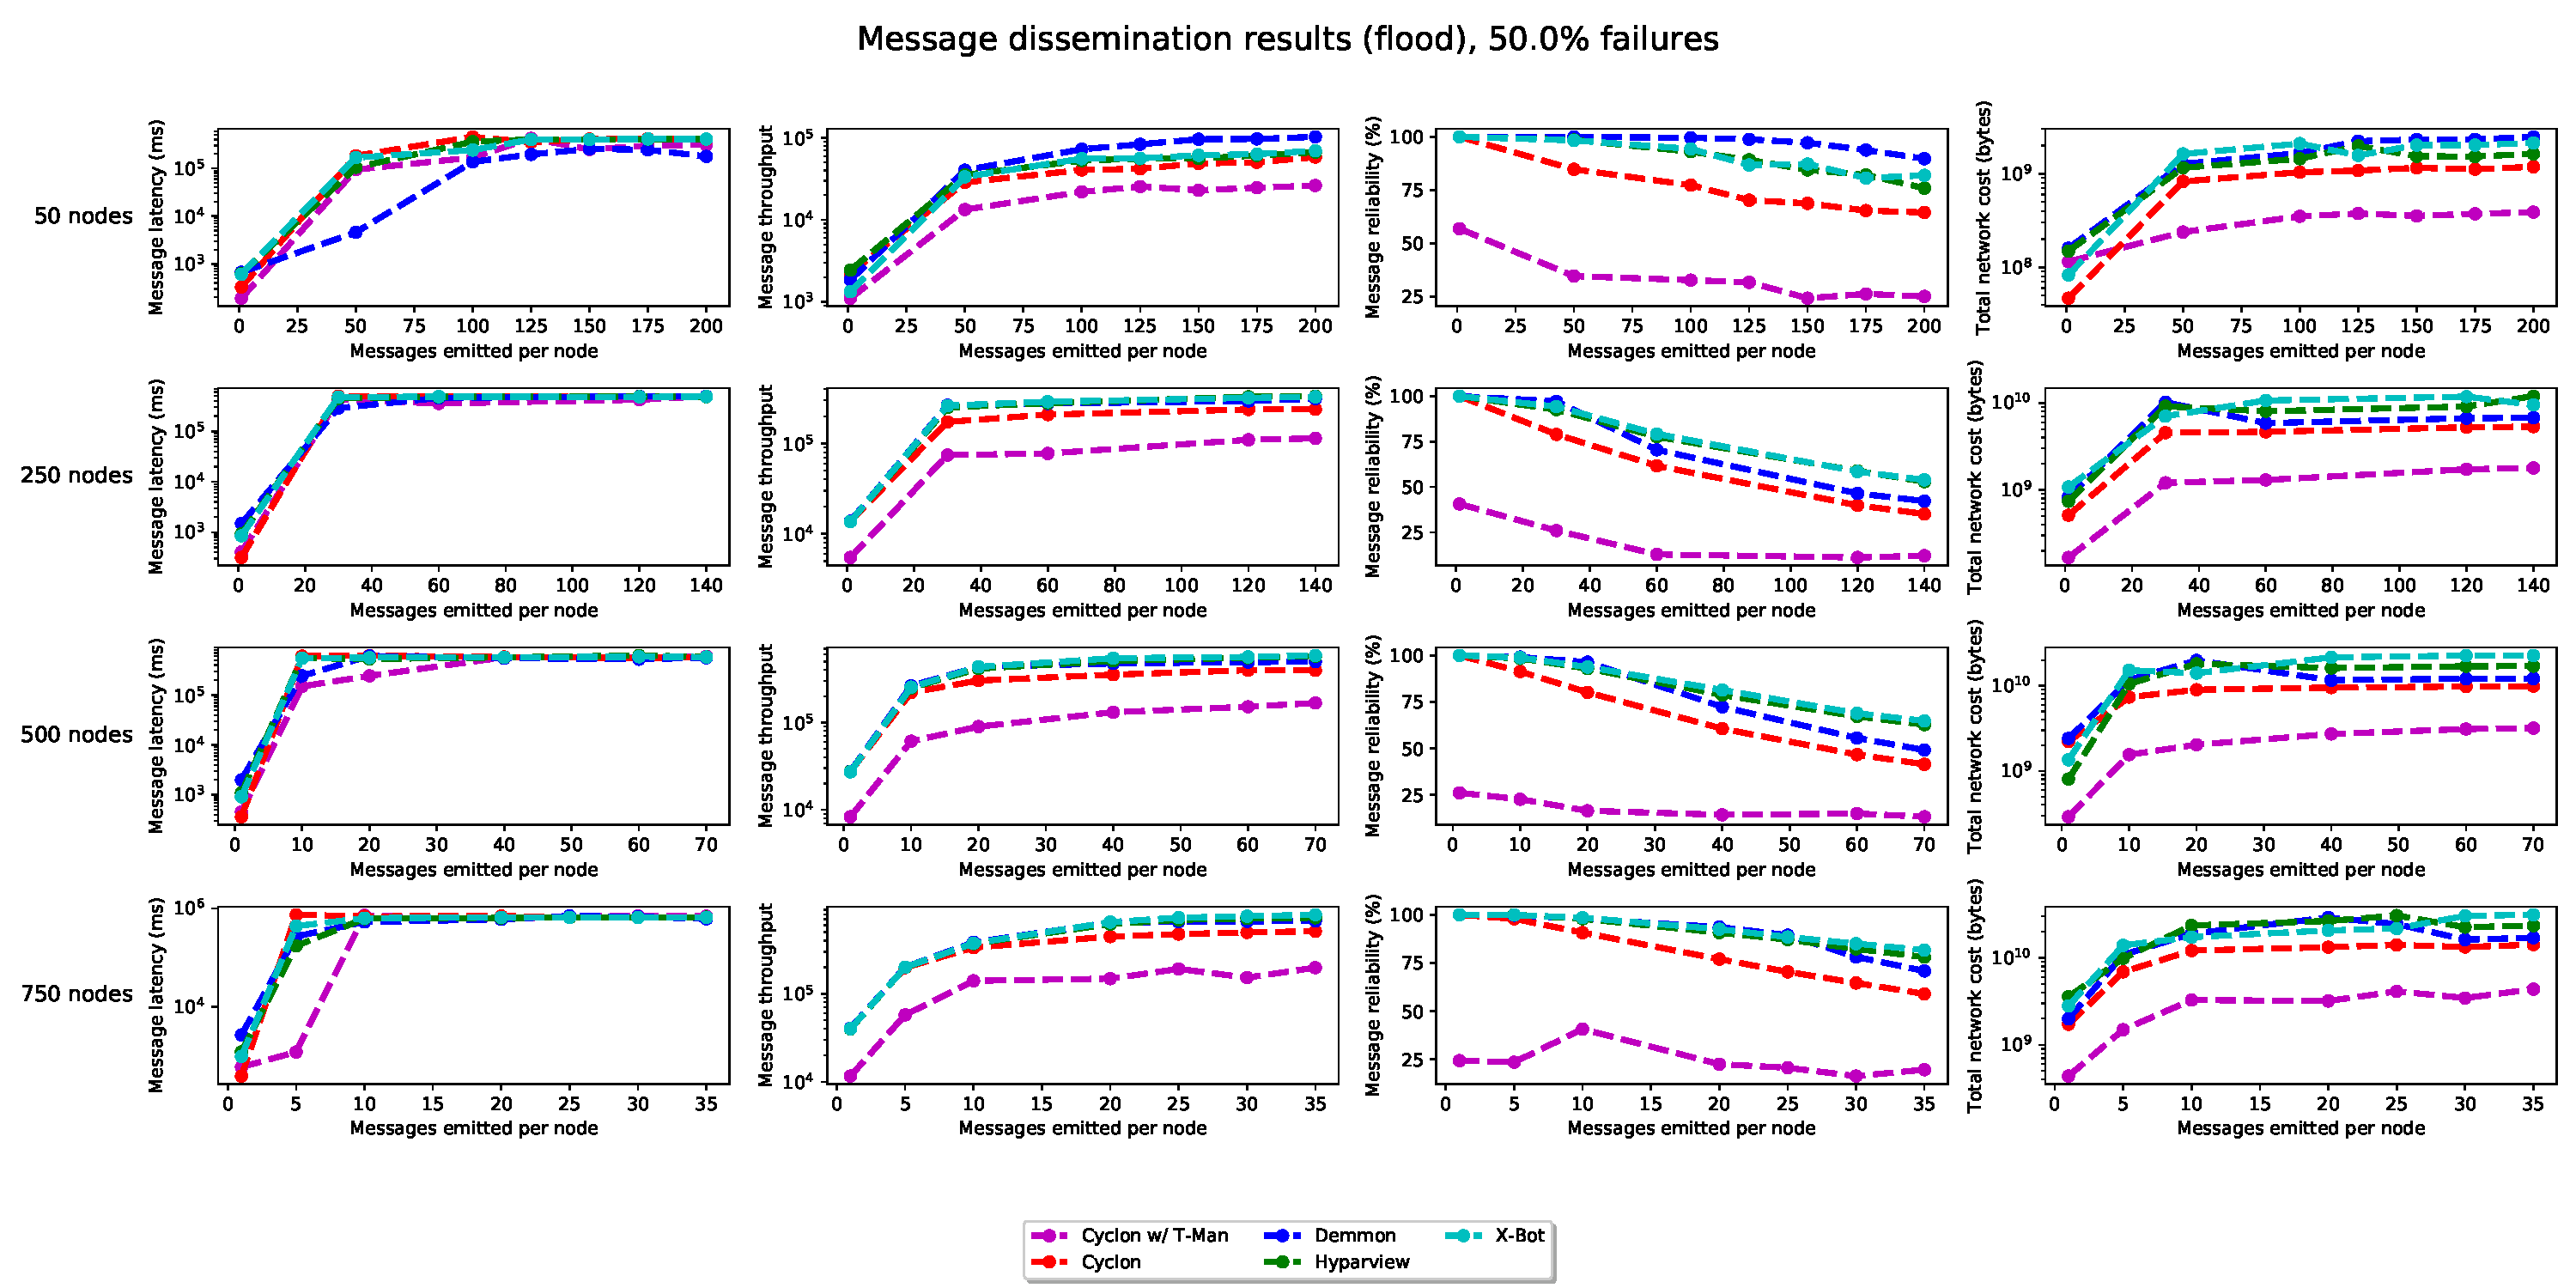
\includegraphics[width=\columnwidth]{Chapters/evaluation/figures/flood/flood_50.0_failures.pdf}
    \caption{Obtained results in simple flood scenario (50\% failures)}
    \label{fig:pouchbeasts-overview}
\end{figure}

\begin{figure}[htbp]
    \centering
    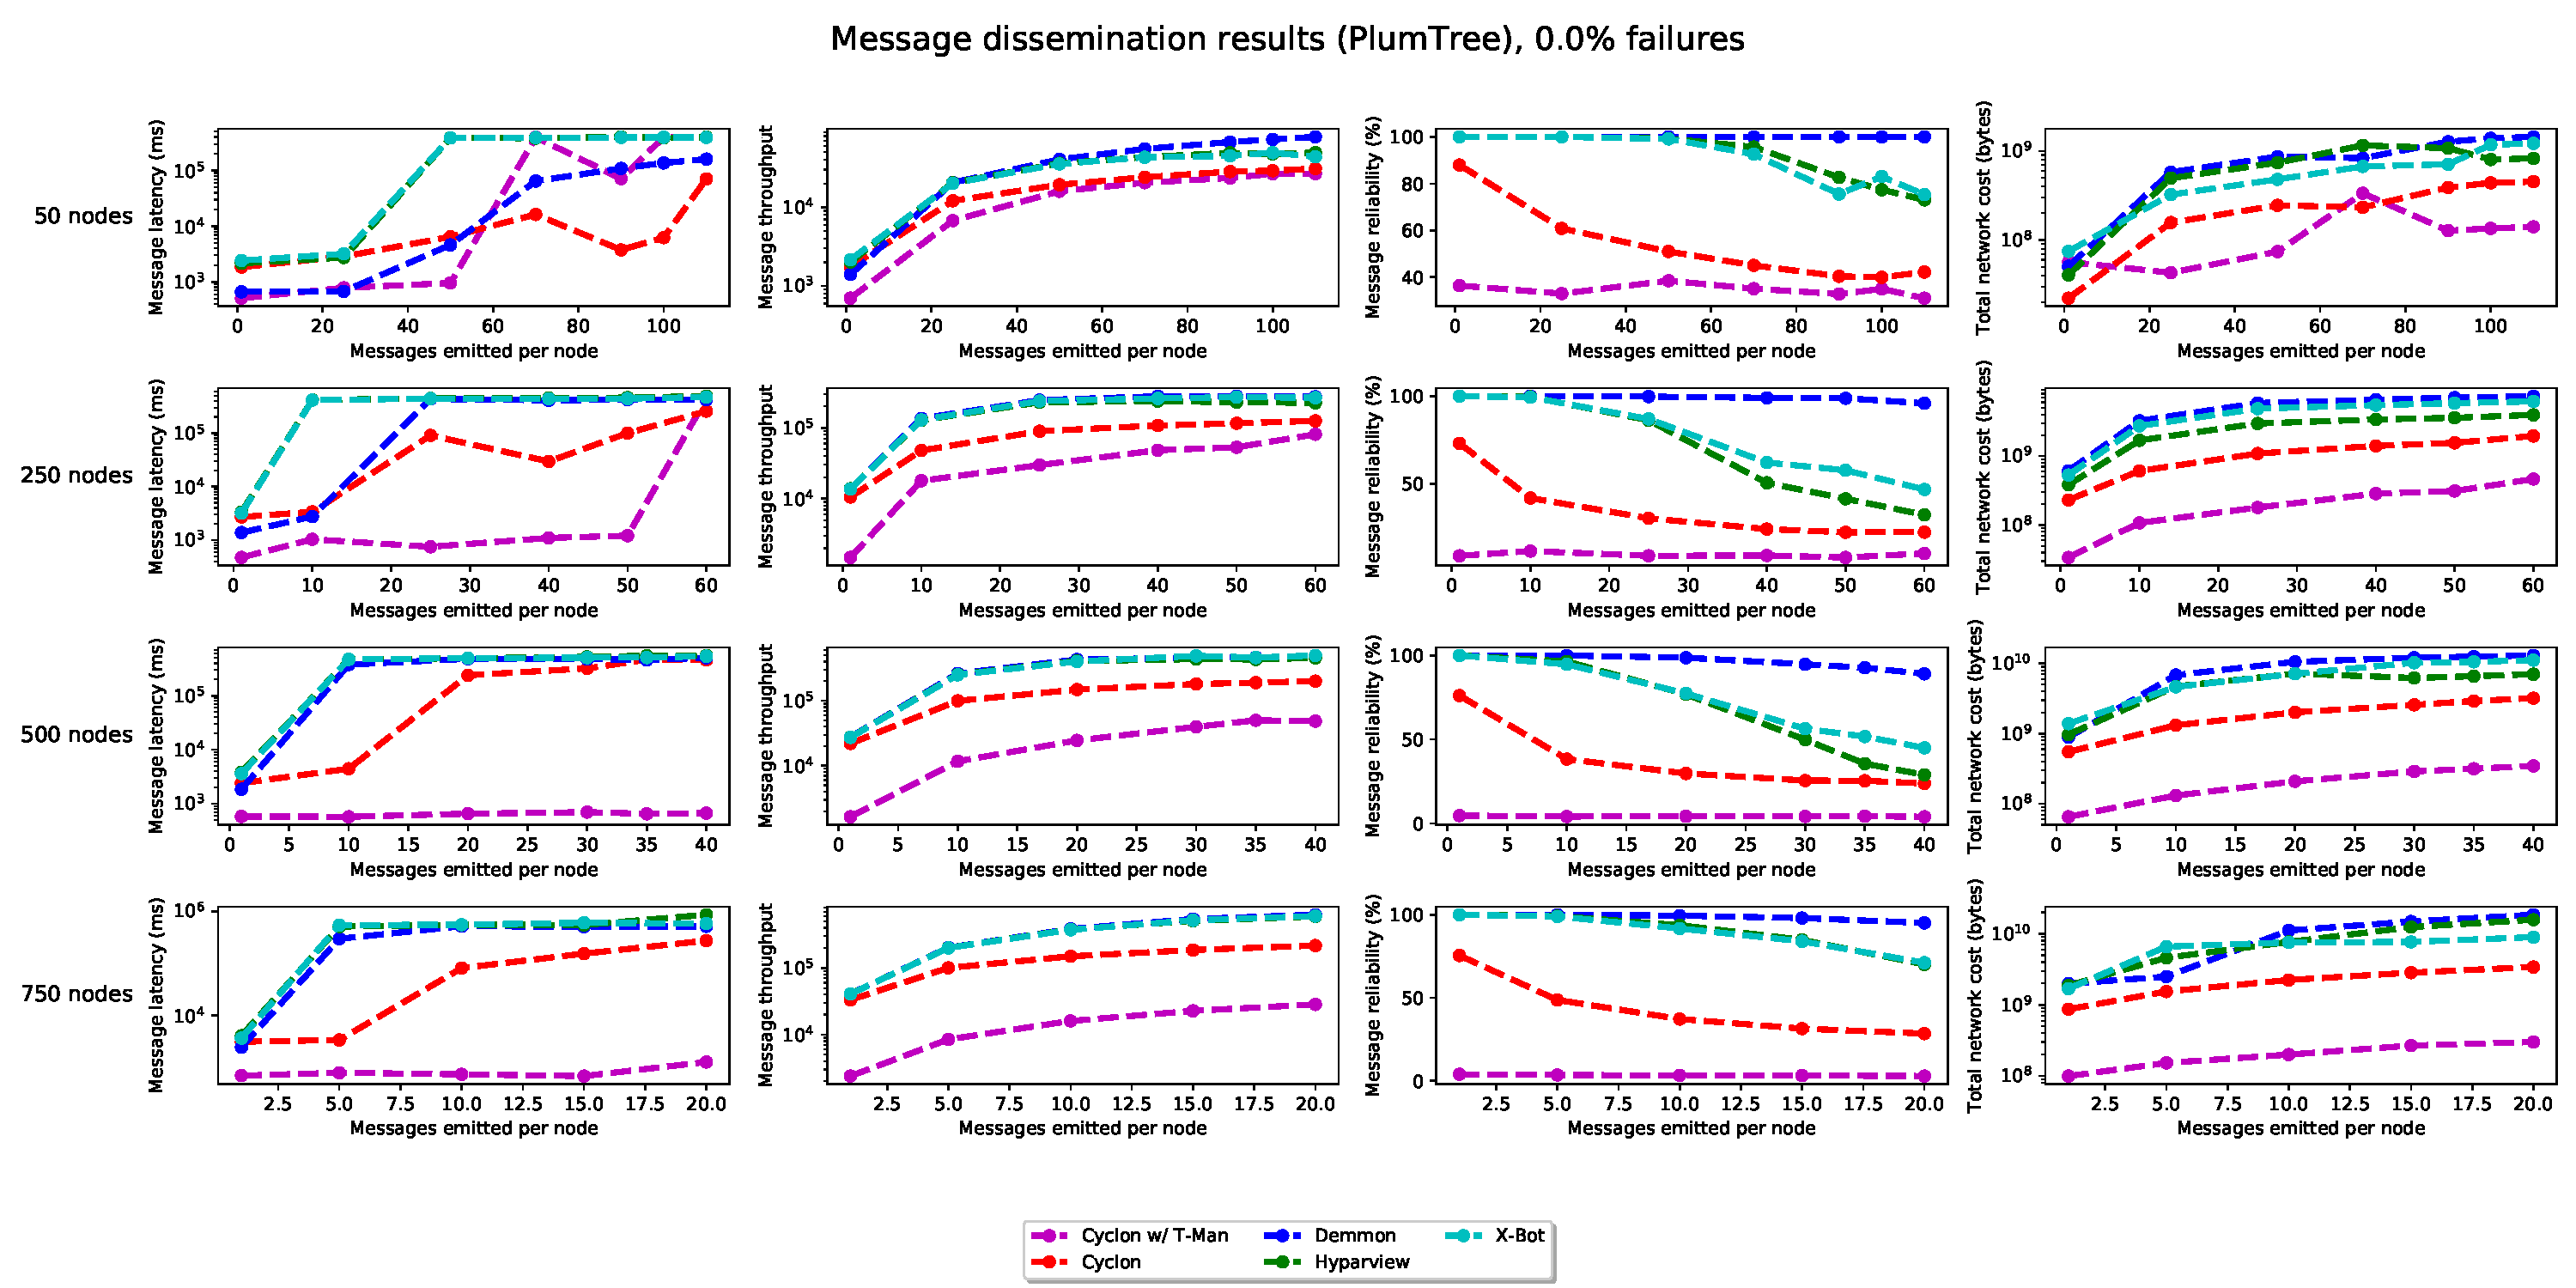
\includegraphics[width=\columnwidth]{Chapters/evaluation/figures/flood/plumTree_0.0_failures.pdf}
    \caption{Obtained results in PlumTree scenario (0\% failures)}
    \label{fig:pouchbeasts-overview}
\end{figure}

\begin{figure}[htbp]
    \centering
    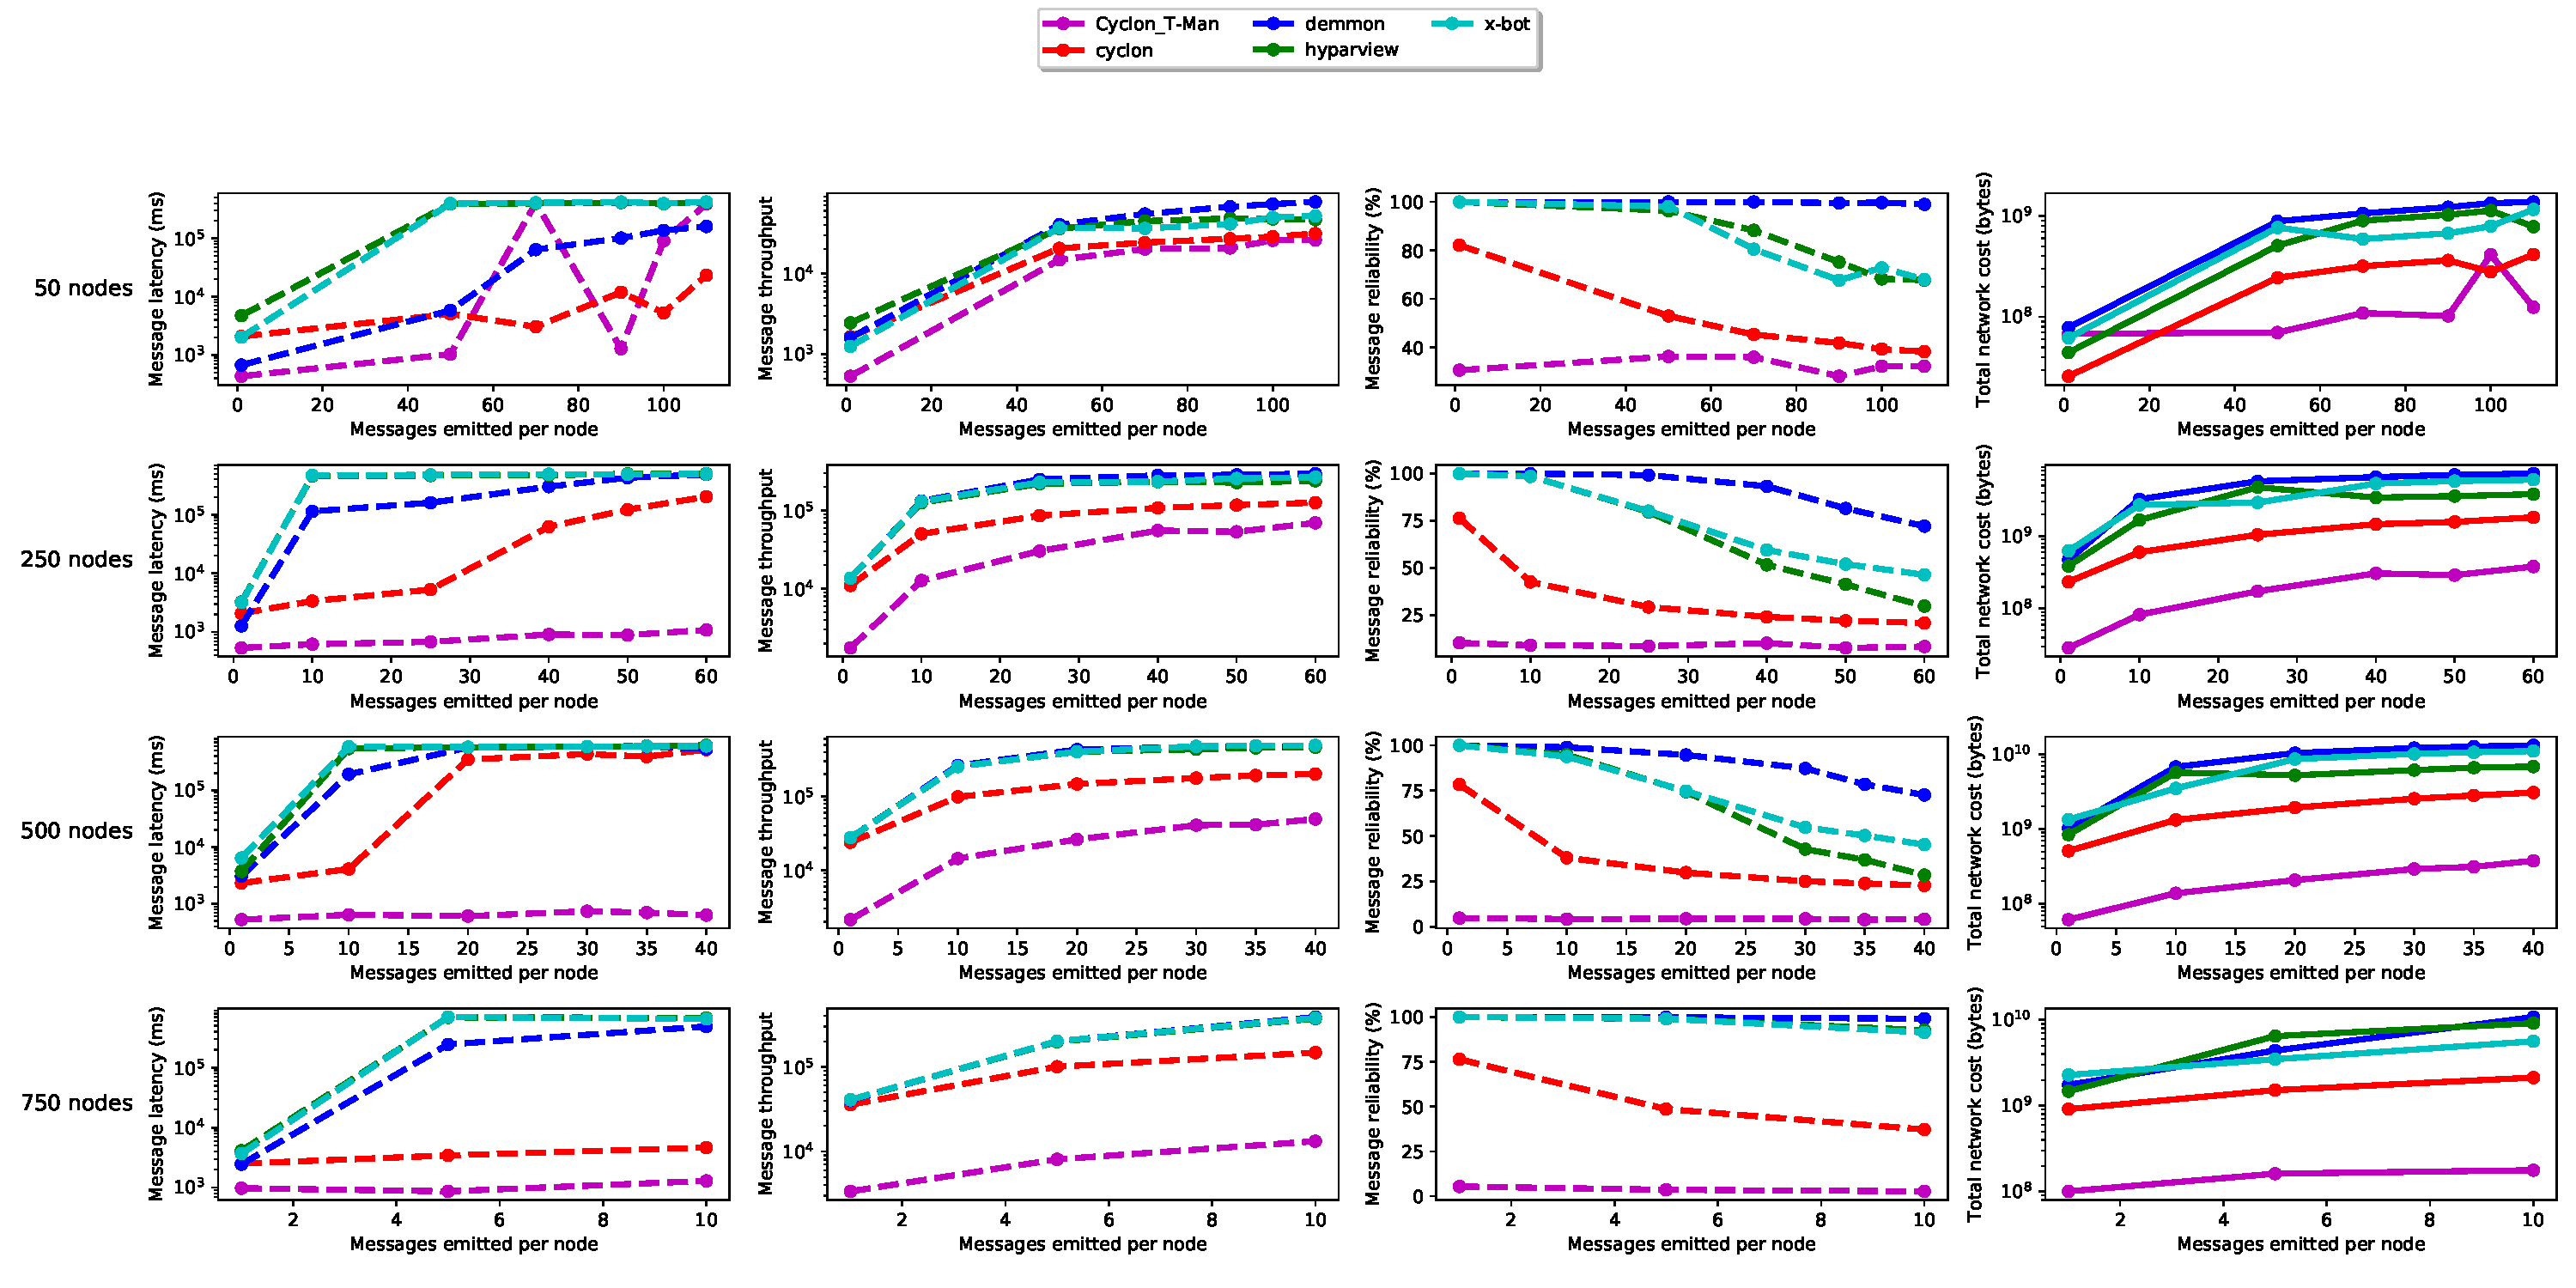
\includegraphics[width=\columnwidth]{Chapters/evaluation/figures/flood/plumTree_50.0_failures.pdf}
    \caption{Obtained results in PlumTree scenario (50\% failures)}
    \label{fig:pouchbeasts-overview}
\end{figure}



\end{landscape}
